\chapter{System Design and Implementation}
\label{ch:method}

\section{Architecture and Project Boundary}

The system is divided into editor, resource, runtime and test components, as shown in Figure \ref{fig:architecture}. The game executes behaviour trees through resource files and runtime components and does not depend on the editor interface. Live Debug also appears only in the Godot editor and is not added to the final game view. The editor interface is integrated through Godot's EditorPlugin extension mechanism, and its node canvas is based on GraphEdit \parencite{godoteditorplugin,godotgraphedit}.

\begin{figure}[htbp]
\centering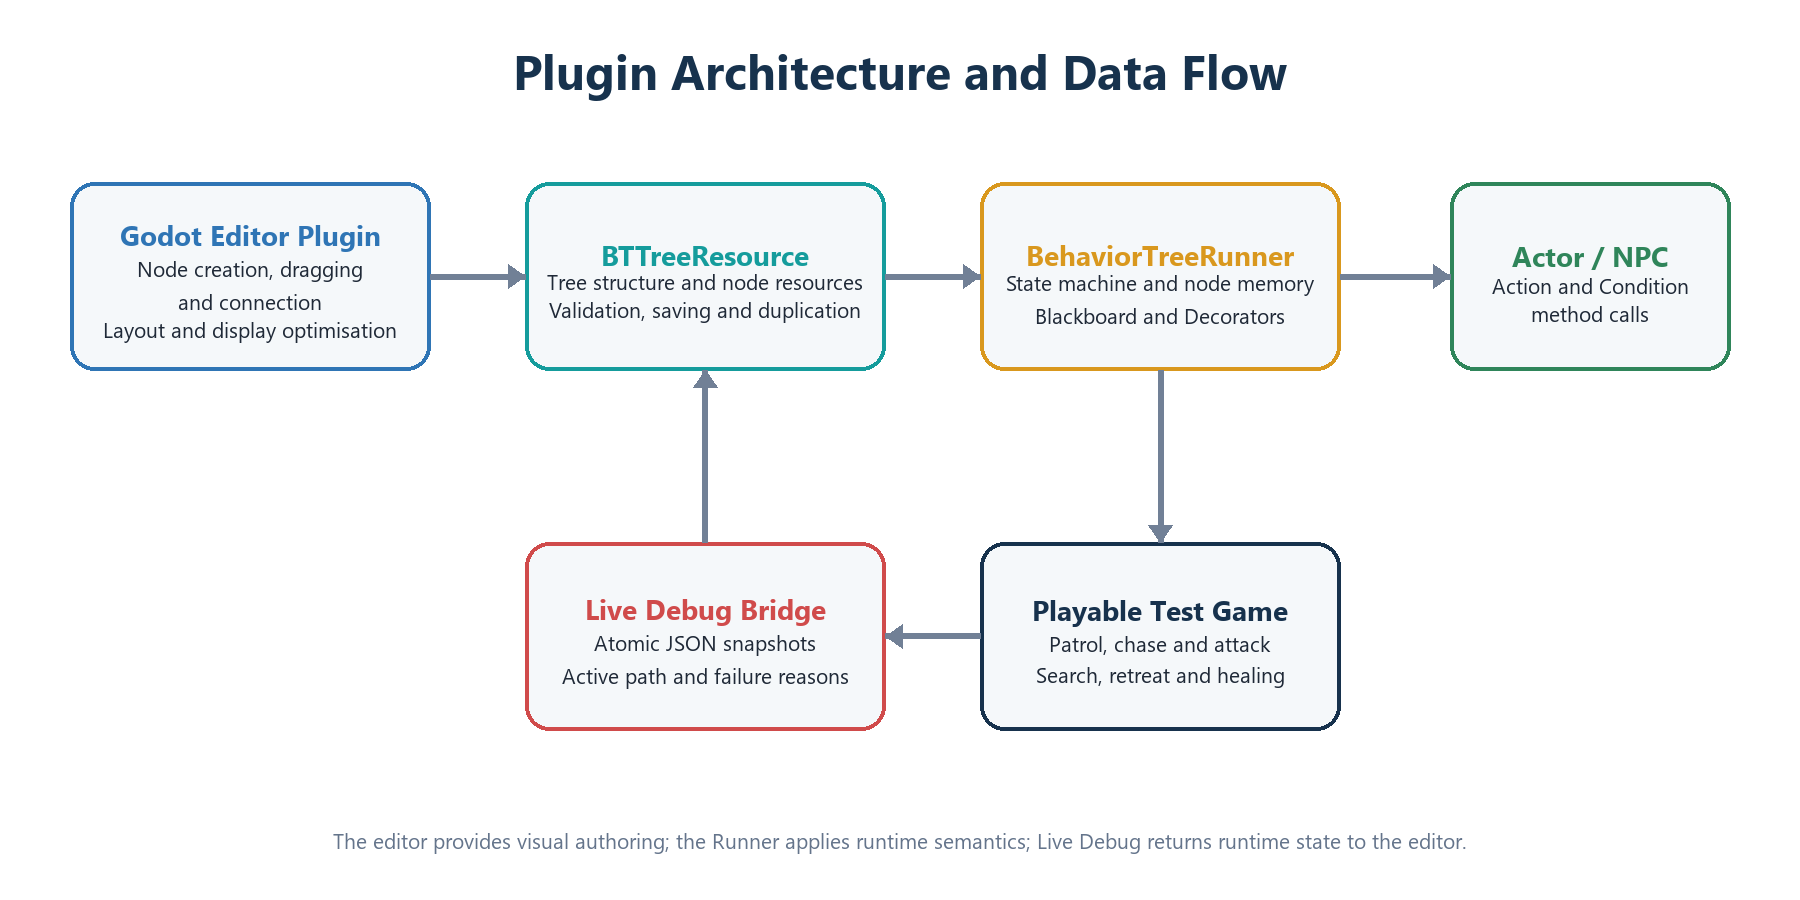
\includegraphics[width=\textwidth]{figures/architecture_en.png}
\caption{Plugin architecture and data flow between the Godot editor, behaviour-tree resource, Runner and Actor.}
\label{fig:architecture}
\end{figure}

\texttt{BTTreeResource} stores the complete tree, while \texttt{BTNodeResource} stores the type, parameters, position and parent relationship of an individual node. \texttt{BehaviorTreeRunner} executes the behaviour tree, and \texttt{BehaviorTreeComponent} connects the tree to an Actor in the scene. The main editor interface is responsible for the canvas, property editing, blackboard, history and Live Debug. This division allows resources, execution logic and the display interface to be tested separately.

\section{Resource Model and Validation}

Ordinary nodes record their parent in \path{parent_id}, while Decorators use a separate \path{decorator_parent_id}. A Decorator is therefore not incorrectly executed as an ordinary child. Sibling nodes are sorted by horizontal position on the canvas, so the visible order from left to right is also the execution order. Node positions and this order are both retained when the resource is saved.

Before saving, the plugin checks that a Root exists, node IDs are not duplicated, parents are valid, Decorators are attached correctly, and node parameters are complete. For example, a Root cannot have a parent, while an Action or Condition cannot own ordinary children. Editor saving and automated testing use the same validation rules.

The blackboard Schema can declare Bool, Int, Float, String and \texttt{Vector2} types and can set a default value for each key. Strict mode reports undeclared or invalid keys. The Inspector provides a key picker while retaining free text input. Schema changes are also included in undo and redo history.

\section{Runtime Semantics}

Every behaviour-tree update returns \textsc{success}, \textsc{failure} or \textsc{running}. Nodes that must continue across frames save progress by ID; these records are cleared when the tree is restarted, replaced or a branch is interrupted. Table \ref{tab:nodes} summarises the behaviour of each node type.

\begin{table}[htbp]
\centering
\caption{Implemented runtime node semantics.}\label{tab:nodes}
\begin{tabular}{p{0.22\textwidth}p{0.68\textwidth}}
\toprule Node & Behaviour \\
\midrule
Root & Executes its single ordinary child.\\
Sequence & Executes children in order, stops on failure or running, and remembers the running index.\\
Selector & Executes children in order, stops on success or running, and remembers the running index.\\
Reactive Selector & Rechecks from the highest priority on every Tick and can interrupt a lower-priority branch.\\
Random Selector & Uses a seedable random choice and retains the same child while running.\\
Parallel & Ticks multiple children and applies success and failure thresholds.\\
Repeat & Repeats a fixed number of times or indefinitely and preserves the count across Ticks.\\
Wait & Accumulates delta and succeeds when the duration is reached.\\
Condition & Calls an Actor predicate or compares a blackboard value.\\
Action & Calls an Actor method and converts a Bool or status into a tree state.\\
\bottomrule
\end{tabular}
\end{table}

Action and Actor-mode Condition nodes call Actor methods through a common interface. If a method does not exist, the node returns failure and displays the reason instead of crashing the game. Blackboard conditions support key existence, truth, equality, inequality and numeric comparison.

Decorators change a condition or result before or after their owner node executes. Implemented behaviours include blackboard comparison, cooldown, time limit, result inversion, forced result and repetition. Resetting a subtree clears the saved execution progress of both Decorators and child nodes.

\section{Editor Authoring Workflow}

The plugin is displayed in the bottom panel of the Godot editor. Users right-click the canvas to create a node and do not need to face a row of creation buttons in the menu bar. Nodes can be moved, connected, disconnected, duplicated and deleted. The behaviour-tree selector displays only resource names, so users do not need to view or enter complete file paths manually. Creation, deletion, movement, connections, parameter changes, Schema changes and collapsed state all support undo and redo.

The Inspector uses controls corresponding to field types. For example, an Action directly enters a method name, while a Condition selects Actor or blackboard mode and sets a key, comparison and value. Random, Parallel, Repeat, Wait and Decorator nodes also have their own settings. Advanced JSON is retained only as a compatibility entry and is not required for normal operation.

The plugin uses connection ports above and below nodes, whereas Godot's default connections are mainly designed for left and right ports. The plugin therefore draws the final connections itself while using Godot's preview when a connection is dragged. Custom connections can still be disconnected with a right click and support undo and redo. Disabling custom display restores Godot's native connections.

\section{Live Debug and Blackboard Inspection}

At runtime, the current Actor, behaviour tree, active node, execution path, failure reason and blackboard values are written to a debug file. The old version is replaced only after the file has been completely written, preventing the editor from reading incomplete content. If one read fails, the editor retains the previous complete state and retries on the next update.

The editor displays debugging information only for the current behaviour tree. The active path uses a prominent border, inactive branches can be dimmed, failed nodes display a reason, and the blackboard panel displays current keys and values. Long paths are placed in a scrollable area to prevent them from covering the main canvas. None of this debugging content appears in the game view. An example is shown in Figure~\ref{fig:livedebug}.

\begin{figure}[htbp]
\centering
\includegraphics[width=0.92\textwidth]{figures/07_runtime_failure.png}
\caption{Editor-only display of the active path and failure reason.}\label{fig:livedebug}
\end{figure}

\section{Large-Tree Display Mechanisms}

The problem of a large behaviour tree comes not only from node count, but also from the simultaneous growth of card information, connection density, navigation distance and runtime state. The plugin therefore provides display functions in four areas: information density, focus and structural reduction, navigation and overview, and connection and runtime representation.

\subsection{Information-Density Control}
Compact reduces card size without hiding nodes. Cards retain the node type and short title, while parameters, descriptions and Decorator summaries can be displayed when needed. Semantic Zoom changes the information level according to the canvas zoom ratio: close views display complete fields, medium views retain titles and key parameters, and distant views retain only the information required to identify nodes. Neither function changes the behaviour-tree resource.

Node types are also redundantly encoded with colour, icons and shapes. Even when colours are difficult to distinguish, users can identify the Root, composite nodes, tasks and Decorators through icons and outlines. The plugin also provides a colourblind-safe palette, reducing reliance on a single colour channel. The two information-density states are shown in Figure~\ref{fig:compact}.

\begin{figure}[htbp]
\centering

\includegraphics[width=0.92\textwidth]{figures/01_baseline.png}
\par\smallskip{\small (a) Baseline}\par\medskip

\includegraphics[width=0.92\textwidth]{figures/02_compact.png}
\par\smallskip{\small (b) Compact cards}
\caption{Full-detail Baseline and Compact Cards for the same behaviour tree.}\label{fig:compact}
\end{figure}

\subsection{Focus and Structural Reduction}
Fisheye Focus+Context enlarges cards near the pointer while retaining surrounding nodes as positional references. Maximum magnification is limited to 1.20 times, and card positions are compensated around their own centres to prevent the overall layout from drifting continuously after magnification. When fisheye is disabled, cards return to their original size and position.

Search supports the title, type, description and parameters of Action, Condition and Decorator nodes, and provides previous, next and clear operations. Matching nodes remain prominent, other nodes are dimmed, and the selected target can be moved into the current viewport. Subtree Focus displays only the specified branch and necessary context; Context Collapse retains the collapsed root and a summary of hidden nodes but temporarily does not draw descendants. After expansion, the original node positions and parent--child relationships are still used. Fisheye and collapse examples are shown in Figure~\ref{fig:focuscollapse}.

\begin{figure}[htbp]
\centering

\includegraphics[width=0.92\textwidth]{figures/03_fisheye.png}
\par\smallskip{\small (a) Fisheye focus and context}\par\medskip

\includegraphics[width=0.92\textwidth]{figures/05_collapsed.png}
\par\smallskip{\small (b) Subtree collapse and summary}
\caption{Two implementations of local magnification and structural reduction.}\label{fig:focuscollapse}
\end{figure}

\subsection{Navigation and Overview}
The enhanced minimap uses a fixed area to display a reduced structure of the complete tree and marks the current viewport position. Fit moves the current graph into a visible range, Focus locates the selected node, and Show All cancels a partial display and returns to the complete tree. Breadcrumb displays the hierarchical path from the Root to the current node, while the path summary states the current execution or selection path in text, allowing the current location to remain identifiable when cards are reduced.

Search results can be traversed with buttons or the keyboard. Multi-column layout separates branches with many children into multiple columns to avoid unlimited horizontal expansion on one level; stable layout attempts to retain the positions of unmodified branches and reduce widespread movement caused by a single edit. Automatic arrangement still preserves the left-to-right execution order of siblings. The related navigation controls are shown in Figure~\ref{fig:navigation}.

\begin{figure}[htbp]
\centering
\includegraphics[width=0.92\textwidth]{figures/10_complex_tree.png}
\caption{Minimap, path summary, navigation controls and automatic layout in a complex tree.}\label{fig:navigation}
\end{figure}

\subsection{Connection and Runtime Representation}
The plugin uses an output port below a node and an input port above it to express a parent--child relationship. Final connections are drawn by the plugin, while the drag preview continues to use Godot GraphEdit input handling. Orthogonal connections use horizontal and vertical segments to reduce curve crossings; edge bundling first gives connections with a common parent a shared trunk and then branches towards each child. Both methods retain connection clicking, disconnection, undo and redo.

The runtime representation displays the active path, current node, success or failure state, inactive-branch dimming and failure reason on the same canvas. Path colour propagates continuously along parent--child relationships, and a Decorator failure is displayed near its owner node. Users can therefore see both the static structure and the branch actually traversed by the current Tick. Connection and runtime-state examples are shown in Figure~\ref{fig:edgesruntime}.

\begin{figure}[htbp]
\centering

\includegraphics[width=0.92\textwidth]{figures/08_orthogonal_edges.png}
\par\smallskip{\small (a) Orthogonal connections and active path}\par\medskip

\includegraphics[width=0.92\textwidth]{figures/09_bundled_edges.png}
\par\smallskip{\small (b) Edge bundling and failure annotation}
\caption{Connection organisation and runtime-state representation.}\label{fig:edgesruntime}
\end{figure}

\section{Physical Screen Experiment Infrastructure}

The screen-testing tool reads physical width and height from EDID and records them separately from resolution. For a screen of width \(W_{\mathrm{cm}}\) and height \(H_{\mathrm{cm}}\), the test canvas is
\[
W_c=35W_{\mathrm{cm}}, \qquad H_c=35H_{\mathrm{cm}},
\]
where \(W_c\) and \(H_c\) are the logical width and height of the canvas. Every screen uses 35 logical units per centimetre, so the experiment compares physical display area rather than the pixel density of different devices.

The test window moves to the specified screen and then loads the same behaviour tree and display condition. Every test saves device information and raw CSV data. When a new screen is connected in the future, its data are written to a new Session without overwriting existing results.

\section{Demonstration Game}

The complex two-dimensional arena confirms that the behaviour tree can control actual game enemies. The player can move, jump, climb, perform a melee attack, dash, heal and become briefly invisible. Three guards share the same 241-node behaviour tree. According to distance, health, obstacles and player state, guards select defence, melee attack, ranged attack, jumping, climbing, pursuit, search, retreat, healing, patrol or idle behaviour.

An enemy detects the player within 330 pixels and abandons the target only when the distance exceeds 460 pixels. Using two different distances prevents the enemy from switching state repeatedly near a boundary. The game uses simple graphics so that development remains focused on behavioural logic and test stability.
